\chapter{Installeren van de practicum omgeving} \label{app:instal}


\hypertarget{chp:vnc}{}
\section{De VNC viewer}
\label{sec:vnc}
Installeer \href{https://www.realvnc.com/en/connect/download/viewer/}{VNC Viewer} op je laptop. Op de RockPi is VNC Server al geïnstalleerd.
% (op de image van de school is dit al gebeurd).
\begin{comment}
\begin{enumerate}
	\item sudo raspi-config
	\begin{itemize}
		\item Kies 3 Interface Options.
			\begin{itemize}
		\item P3 VNC
		 \item Yes
		 \end{itemize}
	 \item 	Kies 2 Display Option.		
	 	\begin{itemize}
	 	  \item D5 VNC Resolutie of D1 Resolution
	 	  \item DM Mode 85 1280x720 of 1280x1024
	     \end{itemize}
	\end{itemize}
\item Start de VNC viewer op, op je laptop. Vul in het scherm \textit{VNC CONNECT}, zie Figuur \ref{fig:winvnc}, het IP adres van de Raspberry PI in.
	\begin{figure}[h!]
	\captionsetup{justification=centering}
	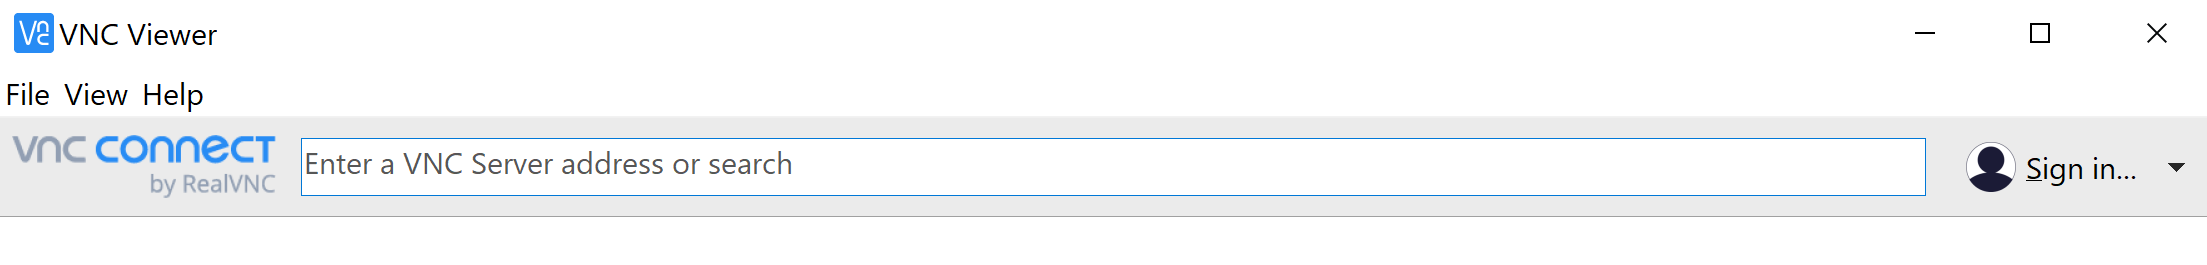
\includegraphics[width=0.7 \linewidth]{figuren/vncopstart}
	\centering
	\caption{Connect met de PI  maken.}
	\label{fig:winvnc}
\end{figure}
Als het goed is krijg je de grafische omgeving van de PI te zien.
\end{enumerate}
\end{comment}
Start op je laptop de VNC viewer op. Vul in het scherm \textit{VNC CONNECT}, zie Figuur \ref{fig:winvnc}, het IP adres van de RockPi in.
\begin{figure}[h!]
	\captionsetup{justification=centering}
	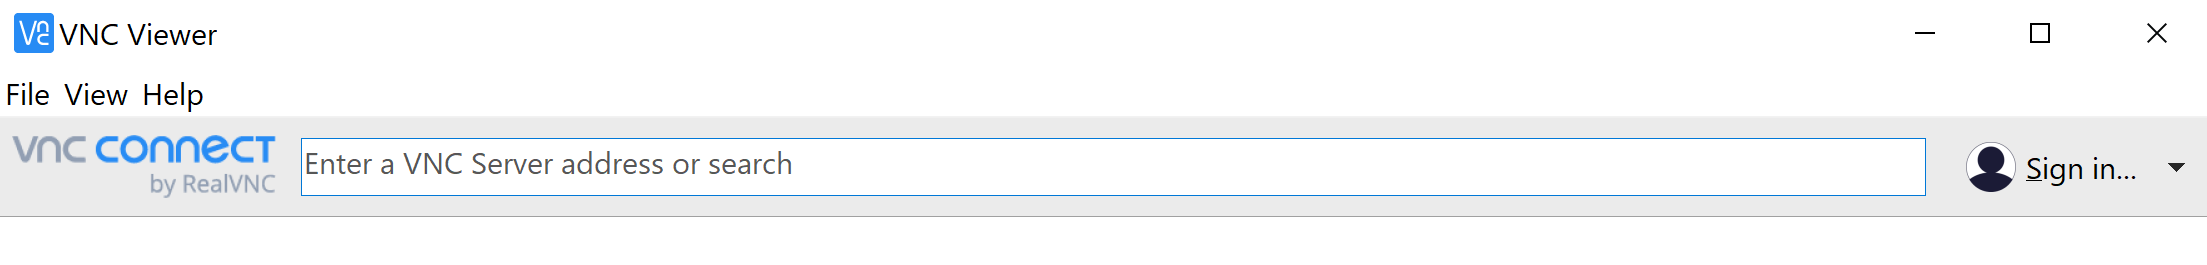
\includegraphics[width=1 \linewidth]{figuren/vncopstart}
	\centering
	\caption{VNC verbinding met de RockPi  maken.}
	\label{fig:winvnc}
\end{figure}
\newline
Als het goed is zie je nu de grafische omgeving van de RockPi. Als dit niet werkt, druk dan eens op de \textbf{'Restart\_X'} knop op het uitbreidingsbordje. Dit herstart de X-Windows grafische schil op de RockPi. Probeer daarna opnieuw te verbinden.

	

\section{Het gebruik van 'Visual Studio Code'} \label{app:vsc}
\label{sec:vsc}
\href{https://code.visualstudio.com/docs}{Visual Studio Code} is een cross platform editor uit de Microsoft omgeving. Je kan vanuit je laptop/desktop omgeving direct files editen op een embedded platform zoals een RockPi. Dit principe is te zien in Figuur \ref{fig:winVCS}.
	\begin{figure}[h!]
	\captionsetup{justification=centering}
	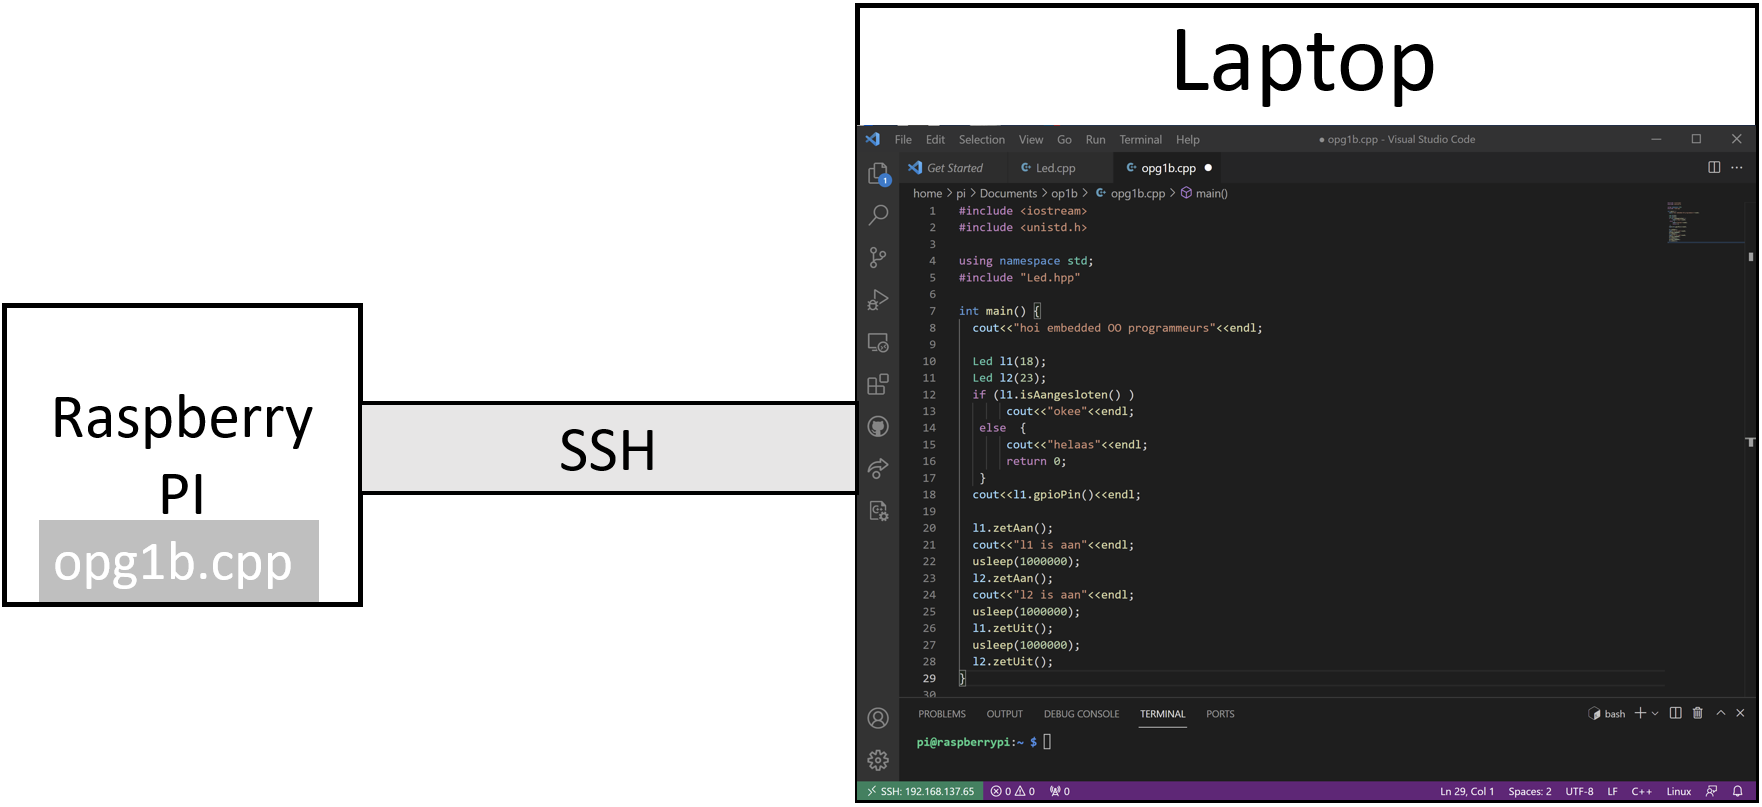
\includegraphics[width=0.65 \linewidth]{figuren/laptopVCS}
	\centering
	\caption{'Visual Studio Code' en de RockPi.}
	\label{fig:winVCS}
\end{figure}
Op de laptop draait 'Visual Studio Code' (VSC) en de source file is de file \texttt{opg1.cpp} op de RockPi. Het compileren kan via VSC, maar kan ook via de terminal in VSC of via een externe terminal b.v Windows PowerShell, KiTTY / PuTTY of een andere.
 

\begin{enumerate}
	\item Download en installeer VCS \href{https://code.visualstudio.com/docs}{Visual studio code}
	\item Bij Visual Studio Code kunnen meerdere extensions geïnstalleerd worden. Het installeren van de \textit{remote SSH} extension kan als volgt gedaan worden:
	\begin{figure}[h!]
	\captionsetup{justification=centering}
	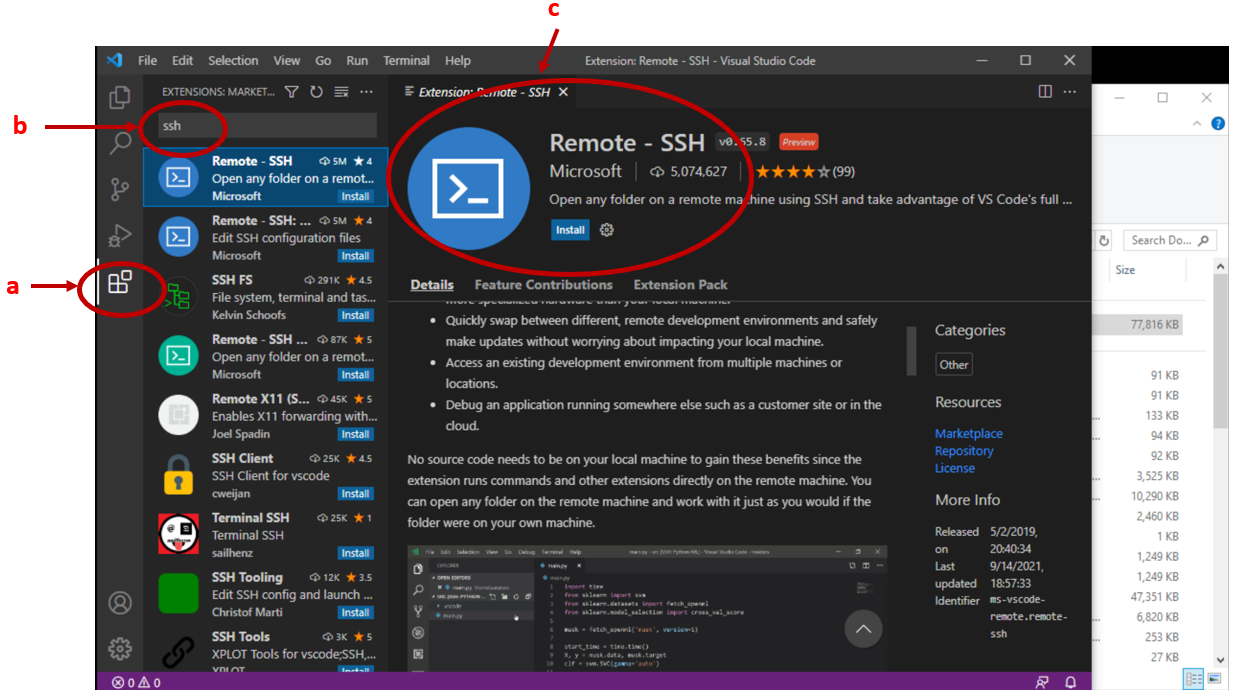
\includegraphics[width=0.6 \linewidth]{figuren/vcsExtSSH}
	\centering
	\caption{Installeren van Remote SSH in VCS.}
	\label{fig:vscEx}
\end{figure}


	\begin{enumerate}
		\item Klik op Extension \img{figuren/extensionIcon} of CTRL + Shift + X
		\item Zoek naar SSH
		\item klik op install
	\end{enumerate}
    \item Verbinding maken met de RockPi.
	\begin{enumerate}
	    \item Ga naar het 'Command Palette' (CTRL+Shift+P). Voer het command Remote-\textcolor{blue}{SSH}:Connect to Host...
	    \begin{figure}[h!]
		\captionsetup{justification=centering}
		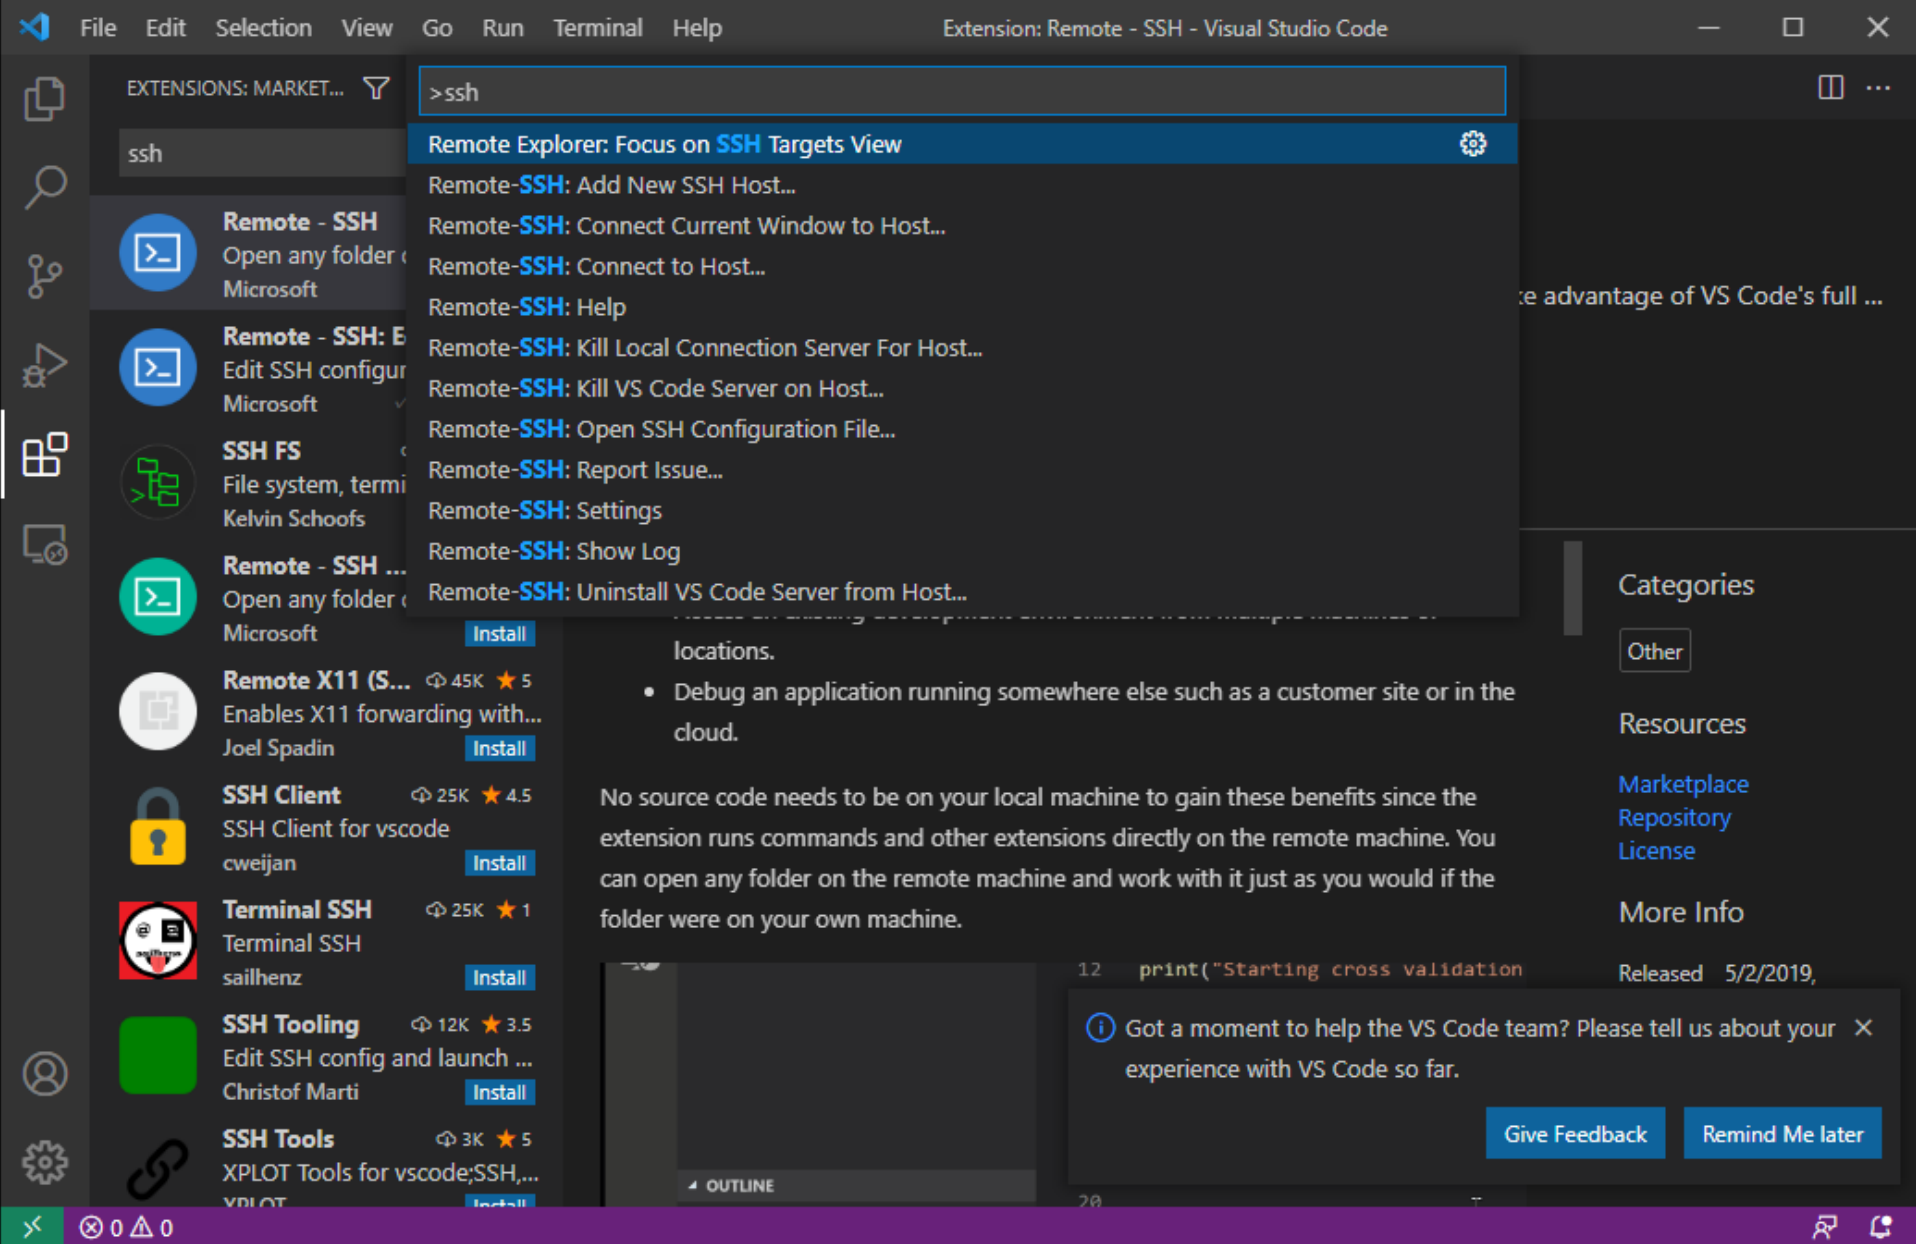
\includegraphics[width=0.6 \linewidth]{figuren/VNCremoteSSH}
		\centering
		\caption{SSH verbinding naar de Host.}
		\label{fig:vscConnect}
	\end{figure}

	Zoals te zien is in Figuur \ref{fig:vscConnect}. VSC komt nu met het scherm zoals te zien is in Figuur \ref{fig:vscAddcon}.
		    \begin{figure}[h!]
		\captionsetup{justification=centering}
		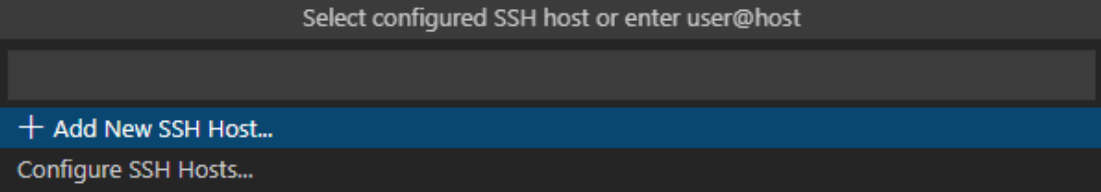
\includegraphics[width=0.6 \linewidth]{figuren/VNCInvoerHost}
		\centering
		\caption{toevoegen van een host.}
		\label{fig:vscAddcon}
	\end{figure}

\item klik op \textit{+ Add New SSH Host}. VSC vraagt vervolgens om een SSH command: type in: ssh rock@\textit{\small{ip.nr. van de host}} zoals te zien is in Figuur \ref{fig:vscConIP}. Uiteraard wel met je eigen IP nummer.
		    \begin{figure}[h!]
	\captionsetup{justification=centering}
	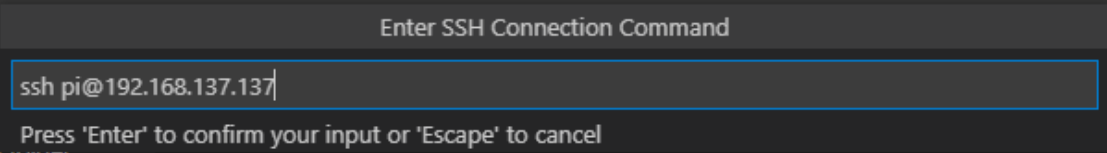
\includegraphics[width=0.7 \linewidth]{figuren/VSCsshCommand}
	\centering
	\caption{connectie maken met de host.}
	\label{fig:vscConIP}
\end{figure}
VSC wil de gegevens opslaan en vraagt vervolgens waar deze opgeslagen moet worden, zoals te zien is in Figuur \ref{fig:vscOpConfig}.
		    \begin{figure}[h!]
	\captionsetup{justification=centering}
	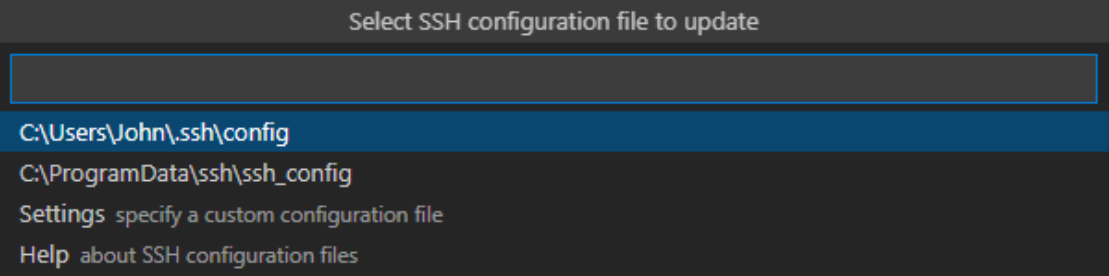
\includegraphics[width=0.7 \linewidth]{figuren/VSCconfigFile}
	\centering
	\caption{waar de gegevens moeten worden opgeslagen.}
	\label{fig:vscOpConfig}
\end{figure}

VSC slaat de gegevens op en geeft een bericht (rechtsonder) of de config file geopend moet worden of dat een connectie gemaakt moet worden. Maak een connectie, VSC komt vervolgens met de vraag of je zeker weet dat je doorgaat, zoals Figuur \ref{fig:vscOpContinue} laat zien.
		    \begin{figure}[h!]
	\captionsetup{justification=centering}
	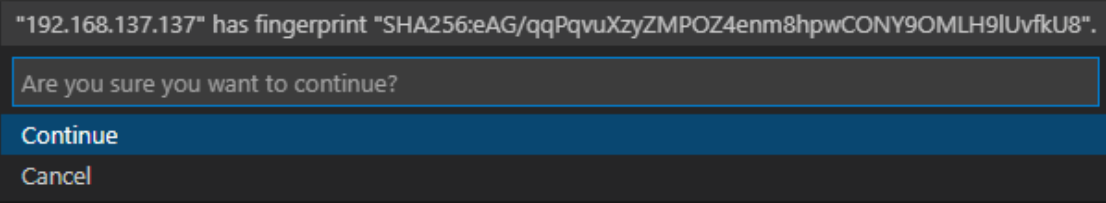
\includegraphics[width=0.7 \linewidth]{figuren/VSCcontinue}
	\centering
	\caption{waar de gegevens moeten worden opgeslagen.}
	\label{fig:vscOpContinue}
\end{figure}

	     \item Klik op \textit{Continue}. VSC vraagt om een password zoals Figuur \ref{fig:vscVrPasswd} laat zien. Het password wordt (of werd) weergegeven op het oled display.
		    \begin{figure}[h!]
	\captionsetup{justification=centering}
	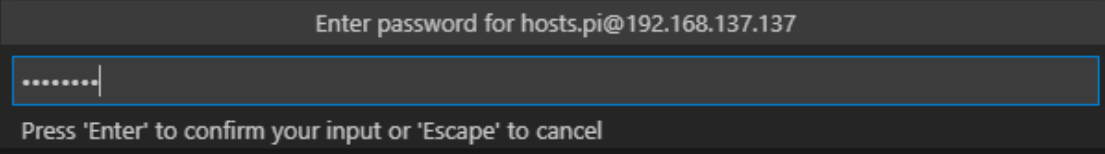
\includegraphics[width=0.7 \linewidth]{figuren/VSCpasswd}
	\centering
	\caption{invullen van een password.}
	\label{fig:vscVrPasswd}
\end{figure}	

Het kan zijn dat een foutmelding gegeven wordt zoals b.v. in Figuur \ref{fig:vscfout1} laat zien. 
		    \begin{figure}[h!]
	\captionsetup{justification=centering}
	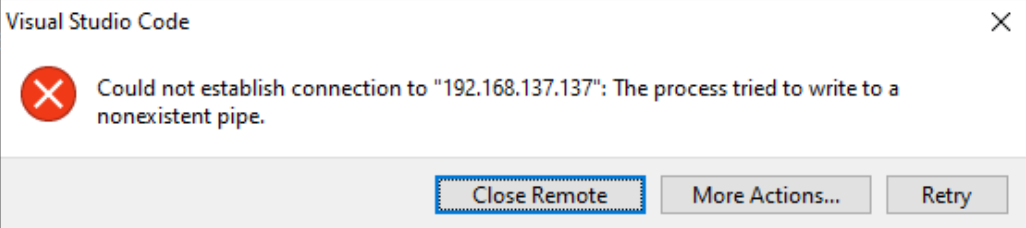
\includegraphics[width=0.6 \linewidth]{figuren/VSCfout1}
	\centering
	\caption{een foutmelding.}
	\label{fig:vscfout1}
\end{figure}	
Raak niet in paniek en probeer desgewenst weer opnieuw.
\item Maak een nieuwe terminal aan (Terminal $\rightarrow$ New Terminal). 
\begin{figure}[h!]
	\captionsetup{justification=centering}
	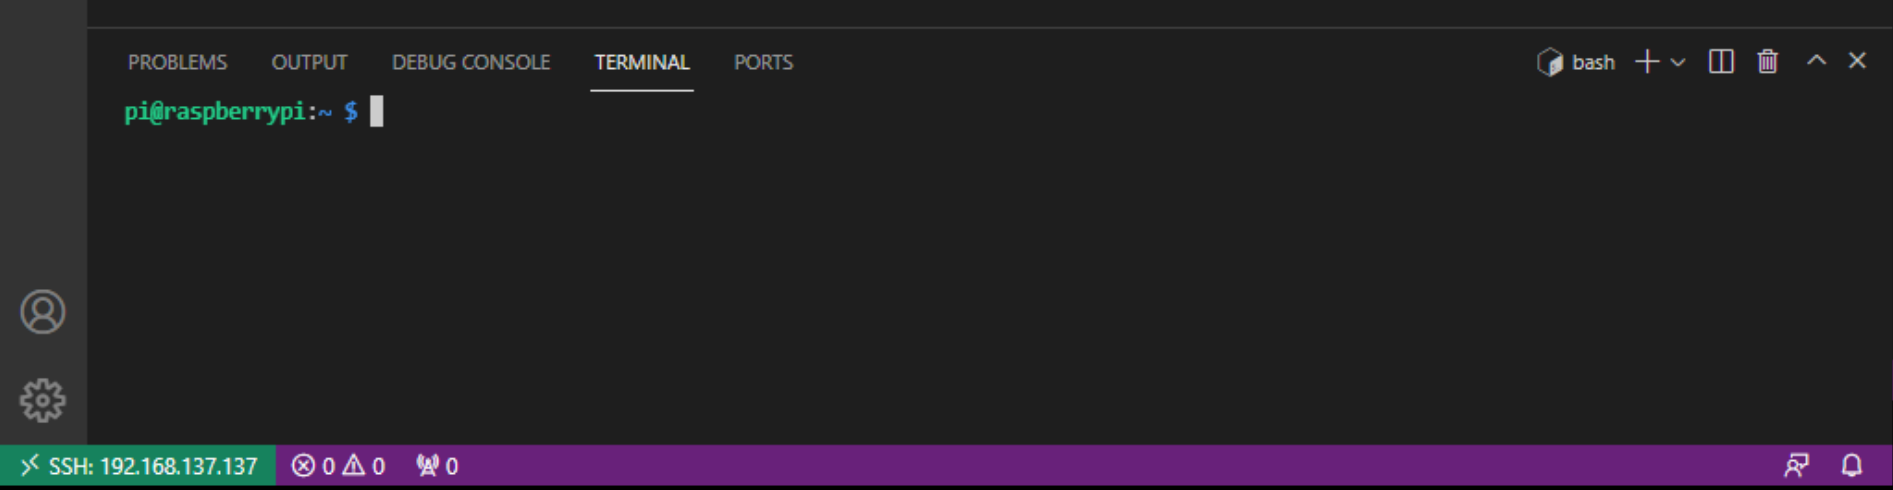
\includegraphics[width=0.6 \linewidth]{figuren/VSCnewTerminal}
	\centering
	\caption{Een geopende terminal in VSC.}
	\label{fig:vscnewTerm}
\end{figure}	
Als het goed is verschijnt de terminal in het onderste deel van VSC met een SSH verbinding naar de RockPi, zoals Figuur \ref{fig:vscnewTerm} laat zien. 
\begin{enumerate}
	\item Met het \textit{ls} commando vraag je de listing op van de huidige directory.
	\item Met het \textit{pwd} commando wordt het pad van de huidige directory zichtbaar.\\
	\textit{pwd} \textless enter\textgreater $\rightarrow$  /home/rock.
	\item  Met het \textit{cd} commando wordt naar een directory gegaan\newline
	(LET OP: Ik ga er van uit dat je een \hyperlink{chp:USBstick}{USB stick} gebruikt!):\\  
	\textit{cd Documents} \textless enter \textgreater $\rightarrow$  
	\textcolor{green}{rock@rockpi-4b}:\textcolor{blue}{$\mathtt{\sim}$/Documents \$}
	\item  Met het \textit{mkdir} commando wordt een directory aangemaakt.\\
	Maak in de directory \textit{Documents} een directory \textit{intro} aan.\newline \\
	Ga naar de directory \textit{intro} (\textit{cd intro}) en vraagt het path op.\\
	\textit{pwd}  $\rightarrow$  /home/rock/Documents/intro
	
\end{enumerate}

\end{enumerate}  
	     \item Het eerste programma op de RockPi.
	     \begin{enumerate}
	     	\item VSC werkt voornamelijk met directory's (folders). Het openen van een folder in VSC op de RockPi kan door te klikken op Explorer \img{figuren/VSCiconeExpl} of Ctrl+Shift+E. VSC opent een scherm, zoiets als \textcolor{red}{\textbf{[1]}} in Figuur \ref{fig:vscOpenFolder}.
		    \begin{figure}[h!]
	\captionsetup{justification=centering}
	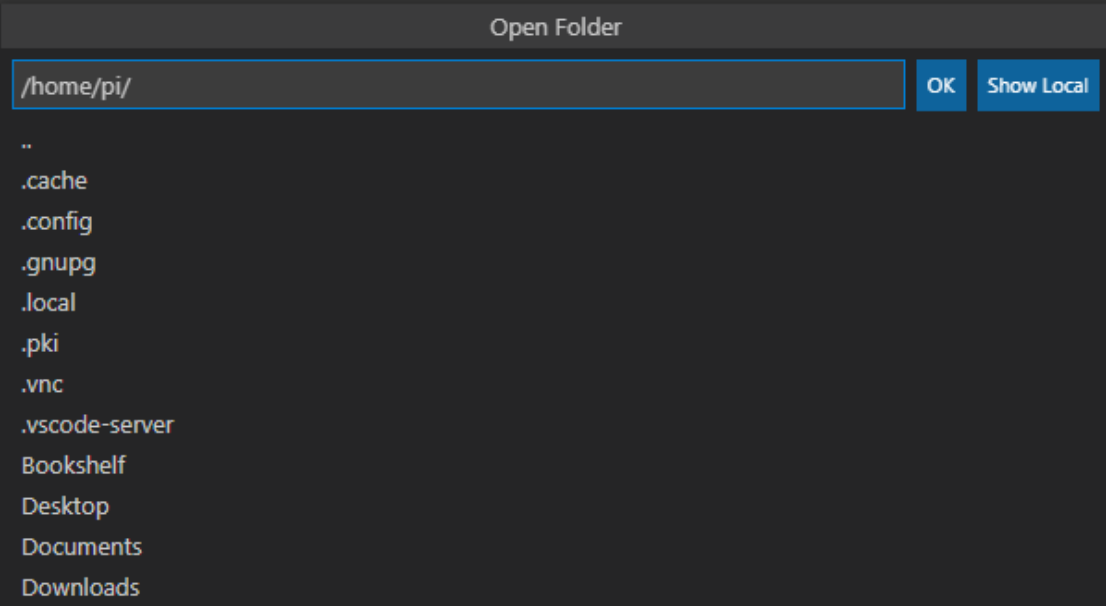
\includegraphics[width=0.8 \linewidth]{figuren/VSCopenFolder}
	\centering
	\caption{De directory die geopend moet worden.}
	\label{fig:vscOpenFolder}
\end{figure}
\newline 
Voer bij \textcolor{red}{\textbf{[2]}} de directory \textit{/home/rock/Documents/intro} in en klik op 'OK'.
VSC kan vragen of je de auteur vertrouwt. Klik op 'Yes'. \\
 In het \textit{EXPLORER} veld verschijnt vervolgens de nu nog lege werkdirectory, zoals in Figuur \ref{fig:vscExploVeld} te zien is.
 	\begin{figure}[h!]
        	\captionsetup{justification=centering}
 	        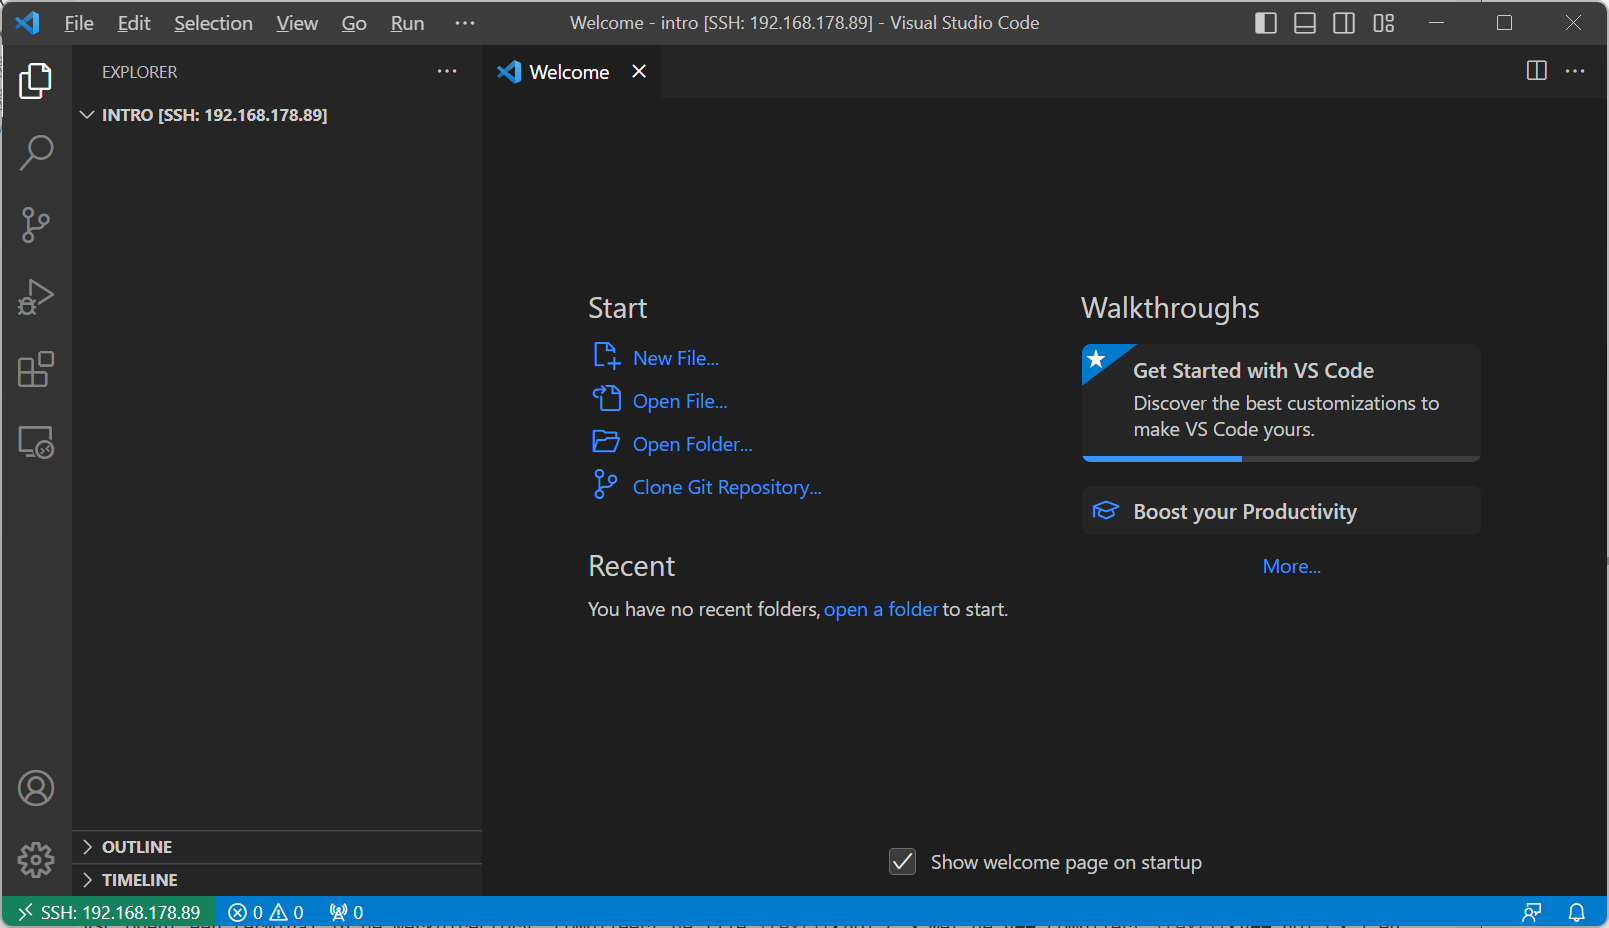
\includegraphics[width=0.6\linewidth]{figuren/VSCexplorerveld}
 	        \centering
 	        \caption{In het EXPLORER veld is de werkdirectory te zien.}
 	         \label{fig:vscExploVeld}
     \end{figure} 
\newpage % Gert
\item Het programma van listing \ref{lst:hoi} kan:  gecreëerd worden door een nieuwe file \textit{hoi.cpp} aan te maken [i], gedownload worden van Brightspace [ii] of gecloned worden van Github [iii].
\begin{enumerate} %{itemize}
 \item
 Klik op New File  \img{figuren/VSCmakeFile} en geef de filenaam \textit{hoi.cpp}.
	 Type/kopieer de tekst van Listing \ref{lst:hoi} in de file \textit{hoi.cpp}
	 
	 \begin{lstlisting}[caption= het meest gebruikte voorbeeld programma.,captionpos=b ,label={lst:hoi}]
#include <stdio.h>
int main(){
	
	printf("Hoi programmeurs van de wereld\n");
	return 0;
}
\end{lstlisting}   	
\item
Download de file \textit{hoi.cpp} van Brightspace en plaats deze in de directory. Het laatste kan zelfs gedaan worden door middel van slepen van de file.
\item
Via git: \textit{git clone~  - -branch intro https://github.com/Johnny63Vi/oopr1.git}\footnote{bij uitvoering geen spatie tussen - -}
Het nadeel van deze methode is dat een directory oopr1 wordt aangemaakt waarin de file komt te staan.
\end{enumerate} %{itemize}

\item Open de bestaande terminal of open een nieuwe terminal \textit{Ctrl+Shift+`}.\newline 
VSC opent een terminal in de werkdirectory. compileer de file \textit{hoi.cpp} met de g++ compiler (\textit{g++ hoi.cpp}) en run het gecompileerde programma \textit{./a.out}.\\
Uiteraard kan ook gekozen worden voor een externe terminal zoals, \textit{Windows PowerShell}, \textit{PuTTY}, etc.\\
Delete a.out (\texttt{rm a.out}). 
	     \end{enumerate}

      \item Compileren via VSC.\\
     Je kan het programma ook via VSC laten compileren.
     
     \begin{enumerate}
     	\item  Daarvoor moet de de C++ omgeving in Visual Studio Code worden geïnstalleerd (is al gedaan bij de RockPi):
     	\begin{enumerate}
     		\item Klik op Extension \img{figuren/extensionIcon} of Ctrl+Shift+X.
     		\item Type in C++ en installeer de C++  \img{figuren/cPlusIcon}, het Extension pack en C/C++ Themes.
        \end{enumerate}
     	\item Activeer het tabblad \textit{hoi.cpp}.
     	\item Klik op \textit{Terminal $\rightarrow$ Configure Default Build Task...}. VSC komt met een scherm zoals Figuur \ref{fig:vscComp}.
\begin{figure}[h!]
	\captionsetup{justification=centering}
	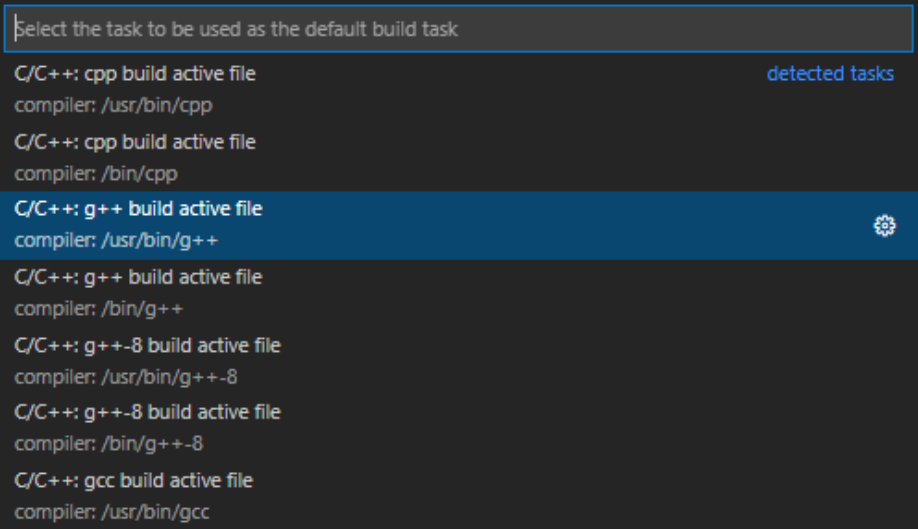
\includegraphics[width=0.6 \linewidth]{figuren/VSCcompile}
	\centering
	\caption{Het kiezen van de compiler.}
	\label{fig:vscComp}
\end{figure}     	
Kies voor \texttt{C/C++: g++ build active file}.
VSC maakt nu een task.json file aan waarin de gegevens betreffende compiler worden opgeslagen.
\item Activeer opnieuw \textit{hoi.cpp} tab. Ga naar Terminal $\rightarrow$ Run Build Task... of \textit{Ctrl+Shift+B}. VSC zal nu \textit{hoi.cpp} compileren.

\item Het gecompileerde programma kan nu gerund worden in b.v. een terminal. Open een terminal of maak een nieuwe terminal aan \textit{Ctrl+Shift+`} en run hoi (\texttt{./hoi}).
\end{enumerate}
     
     \item Run/Debug via VSC.\\
     Je kan een programma ook direct via VSC laten runnen en Debuggen.
     \begin{enumerate}
     	\item Activeer het tabblad \textit{hoi.cpp}.
     	\item Klik op \textit{Run and Debug (Ctrl+Shift+D)} \img{figuren/VSCiconeRunDebug} en vervolgens op\\ \colorbox{NavyBlue}{\textcolor{White}{\textbf{Run and Debug}}}. Afhankelijk van instellingen kan VSC kiezen voor Figuur \ref{fig:kzComp}. 
   Kies hierbij C++ (GDB/LLDB), VSC laat hierna Figuur \ref{fig:kzCompVer} zien. Kies voor: \textit{g++ - Build and Debug active file \small{compiler /usr/bin/g++}}.
   VSC maakt o.a. \textit{launch.json} file aan. Hierin worden diverse gegevens met betrekking tot de compiler/debugger in opgeslagen. \\
   Het zou ook kunnen dat VSC de DEBUG CONSOLE opent. 
      
   \item Klik op tabblad hoi.cpp en plaats vervolgens een breakpoint voor regel 4 (linker muisklik voor regel 4) (printf), een rode stip verschijnt voor de 4. 
   \item Start de debugger:Run $\rightarrow$ Start Debugging of F5 of klik op \img{figuren/VCRrunDebug}. Het programma wordt op de RockPi uitgevoerd en stopt op regel 4, zoals te zien is in Figuur \ref{fig:vscDebugVld}.\newline
\end{enumerate}
     \begin{figure}[h!]
	\centering
	\begin{center} 	
		\begin{subfigure}[b]{0.44\textwidth}
			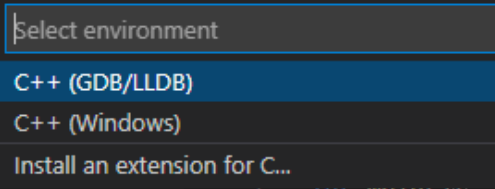
\includegraphics[width=0.85\textwidth]{figuren/VSCksGDB}
			\caption{Keuze welke compiler}
			\label{fig:kzComp}
		\end{subfigure}
		\begin{subfigure}[b]{0.45\textwidth}
			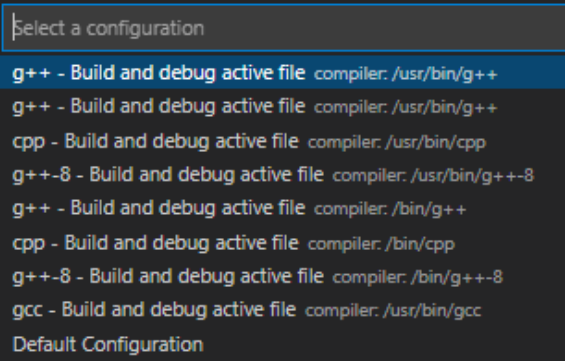
\includegraphics[width=0.95\textwidth]{figuren/VSCKsGcc}
			\caption{Keuze versie compiler}
			\label{fig:kzCompVer}
		\end{subfigure}
		\caption{Keuze compiler te gebruiken door VSC}
		\label{fig:kzcompiler}   
	\end{center}
\end{figure}

\hypertarget{chp:debugknoppen}{}
\begin{figure}[h!]
\captionsetup{justification=centering}
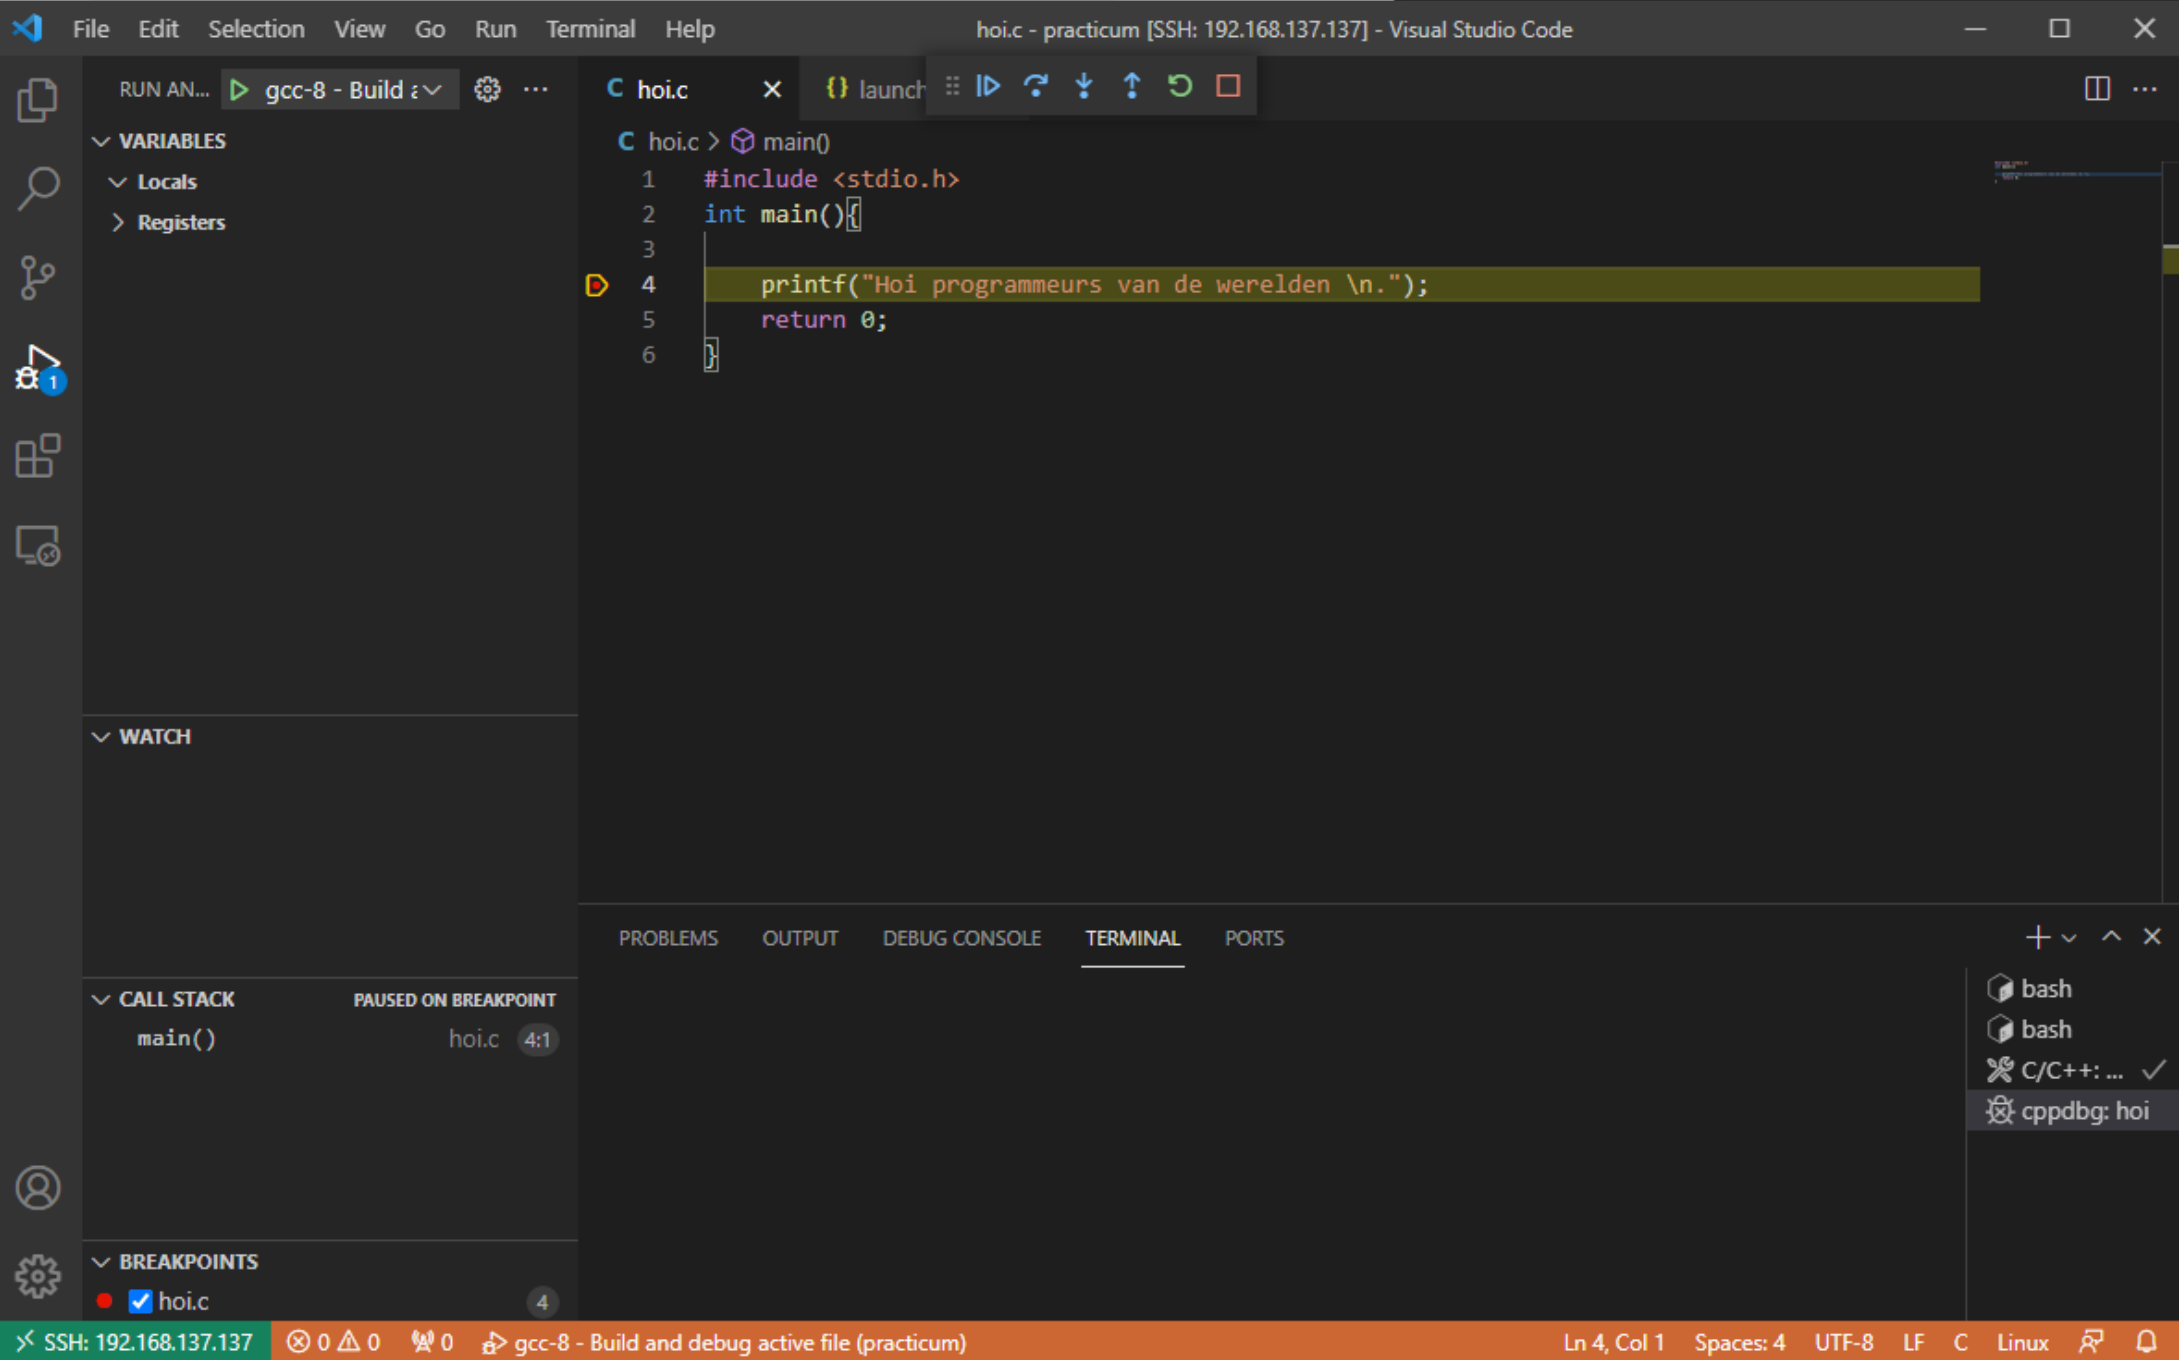
\includegraphics[width=0.8 \linewidth]{figuren/VSCdebugVeld}
\centering
\caption{Debuggen met VSC.}
\label{fig:vscDebugVld}
\end{figure}     
   Met behulp van de debugknoppen 
\includegraphics[width=0.3 \linewidth]{figuren/VSCDebugKnoppen} kan stap voor stap door het programma gelopen worden. Hieronder staan de belangrijkste:

\begin{table}[h!] % [ht]
	\begin{tabular*}{6.6in}{ c | c | l }
		\hline
		
\includegraphics[width=0.05\textwidth, height=8mm]{figuren/F5-Continue} & 'Continue (F5)' & Vervolg het programma zonder onderbrekingen. \\ \hline
		
\includegraphics[width=0.05\textwidth, height=8mm]{figuren/F10-StepOver} & 'Step Over (F10)' & \specialcell{Stap over de volgende regel heen\\(ook als het een functieaanroep is).}  \\ \hline
		
\includegraphics[width=0.05\textwidth, height=8mm]{figuren/F11-StepInto} & 'Step into (F11)' & \specialcell{Voer de regel uit. Als het een functieaanroep is: ga de functie in.\\ \textit{Als het een systeemfunctie is, dan wordt het vaak onbegrijpelijk!}}  \\ \hline
	\end{tabular*}
\end{table}

   
     \end{enumerate}
     
	
